\section{ Laskuvarjokokonaisuus }
\label{laskuvarjokalusto-ja-hyppyvarusteet-laskuvarjokokonaisuus}


\begin{figure*}[]\centering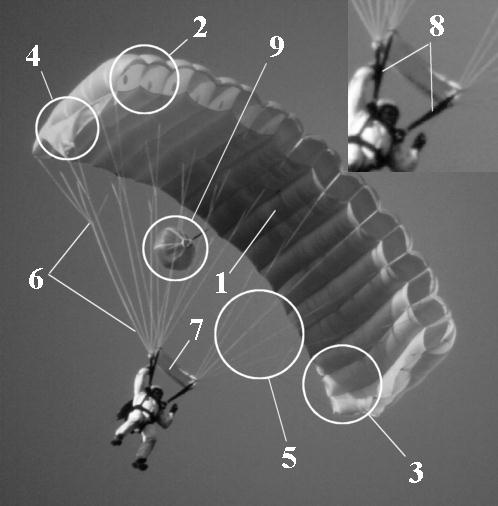
\includegraphics[width=0.7\textwidth]{Paavarjon-osat.jpg}\caption{Päävarjon osat: 1. Kupu 2. Tunnelipari 3. Kuvun takahelma 4. Stabilisaattori 5. Kantopunokset 6. Ohjauspunokset 7. Slider 8. Kantohihnat 9. Apuvarjo}\end{figure*} 


Laskuvarjokokonaisuuteen kuuluu reppu-valjasyhdistelmä sekä kaksi varjoa: pää- ja varavarjo. Molemmat näistä ovat liitovarjoja, jotka ovat muodoltaan siiven kaltaisia. Niiden liitosuhde on noin 3:1, eli liitäessään kolme metriä eteenpäin varjo vajoaa metrin.  


\begin{Figure}\centering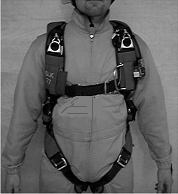
\includegraphics[width=0.7\textwidth]{Reppu-valjas-etu.png}\captionof{figure}{Wings-reppuvaljasyhdistelmä hyppääjän päällä}\end{Figure} 

\subsection{ Päävarjo }
\label{laskuvarjokalusto-ja-hyppyvarusteet-paavarjo}


Päävarjo, joka koostuu kuvusta, punoksista ja sliderista, on kantohihnojen välityksellä kiinni valjaissa kolmirengaslukkojen avulla. Kupu on rakennettu tunneleista, joiden toinen pää on umpinainen. Eripituisilla kantopunoksilla kuvun kohtauskulma pidetään sellaisena, että etureuna on takareunaa hieman alempana. Liitovarjo muodostaa nostovoimaa samalla tavalla kuin lentokoneen siipi. 

\subsection{ Varavarjo }
\label{laskuvarjokalusto-ja-hyppyvarusteet-varavarjo}


Varavarjo on rakenteeltaan ja toiminnaltaan samanlainen kuin päävarjo. Varavarjoa käytettäessä laskeutumispaikka saattaa olla muualla kuin laskeutumisalueella. Tämän vuoksi alastuloasennon on oltava hyvä ja tarvittaessa on tehtävä maahantulokierähdys. 

\section{ Reppu-valjasyhdistelmä }
\label{laskuvarjokalusto-ja-hyppyvarusteet-reppu-valjasyhdistelma}


\begin{Figure}\centering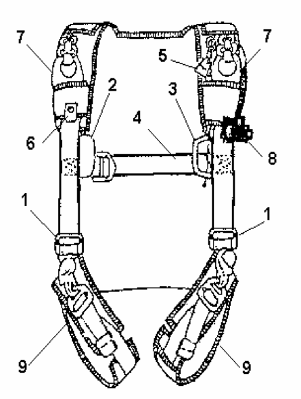
\includegraphics[width=0.6\textwidth]{Reppuvaljasyhdistelma.png}\captionof{figure}{1. Valjaan pystyhihnojen säätösoljet 2. Päävarjon irtipäästöpampula 3. Varavarjon avauskahva 4. Rintahihna 5. Varavarjon pakkolaukaisuhihna RSL 6. Koukkupuukko (sijainti voi vaihdella) 7. Kolmirengasolkalukot 8. FXC-automaattilaukaisimen säätöyksikkö (mikäli käytössä joku muu, merkitse säätöyksikön paikka kuvaan) 9. Reisihihnat}\end{Figure} 


\begin{Figure}\centering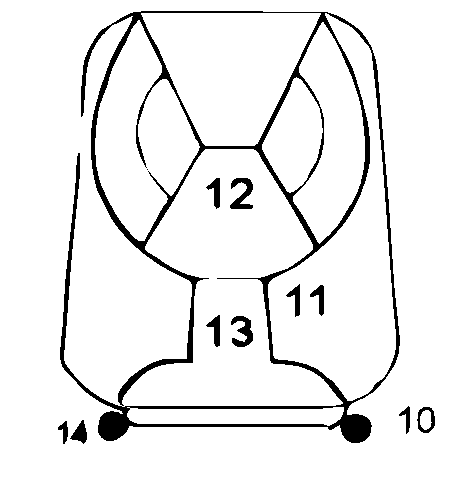
\includegraphics[width=0.6\textwidth]{Reppu-nova.pdf}\captionof{figure}{10. Päävarjon apuvarjo 11. Päävarjon reppu 12. Varavarjon reppu 13. Päävarjon läppä 14. Päävarjon avauskahva hyppymestarille (NOVA-kahva)}\end{Figure} 


\begin{Figure}\centering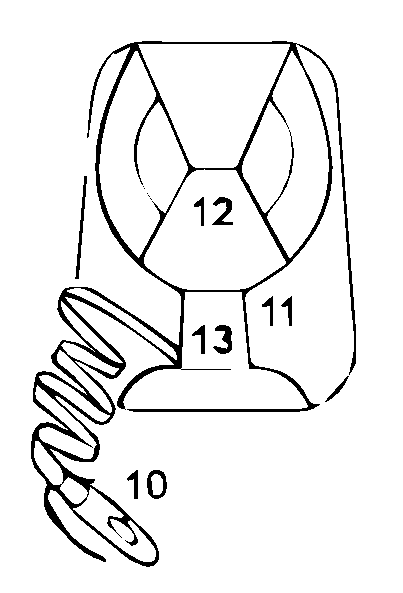
\includegraphics[width=0.6\textwidth]{Reppu-pl.pdf}\captionof{figure}{10. PL-hihna 11. Päävarjon reppu 12. Varavarjon reppu 13. Päävarjon läppä}\end{Figure} 

\section{ Lisälaitteet }
\label{laskuvarjokalusto-ja-hyppyvarusteet-lisalaitteet}


Pää- ja varavarjon lisäksi valjaissa on laitteita lisäämässä hyppääjän turvallisuutta. Näiden laitteiden tarkoituksena on varmistaa varavarjon aukeaminen. 


Varavarjon pakkolaukaisuhihnan (Reserve Static Line, RSL) tarkoituksena on varmistaa varavarjon avautuminen päävarjon irrottua valjaista. Järjestelmä liittää päävarjon kantohihnan ja varavarjon aukaisujärjestelmän yhteen. Hyppääjän on mahdollista vapauttaa varavarjon pakkolaukaisuhihna avaamalla päävarjon kantohihnaan kytketty pikalukko. 


Kun päävarjon kantohihnat ovat päävarjon irtipäästön (\ref{paavarjon-vajaatoiminnot-varavarjon-kaytto} s.\pageref{paavarjon-vajaatoiminnot-varavarjon-kaytto}) jälkeen irronneet kolmirengaslukoista, päävarjo vetää irrotessaan varavarjon pakkolaukaisuhihnasta ja avaa varavarjon. Varavarjon pakkolaukaisuhihna on kuitenkin vain apuväline. Hyppääjän on aina avattava varavarjo vetämällä varavarjon kahvasta! 


\begin{Figure}\centering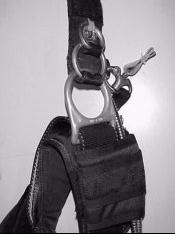
\includegraphics[width=0.7\textwidth]{Kolmirengaslukko.jpg}\captionof{figure}{Kolmirengaslukko}\end{Figure} \begin{Figure}\centering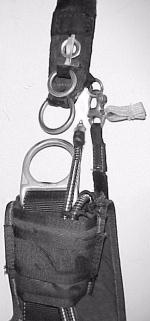
\includegraphics[width=0.7\textwidth]{Kolmirengaslukko-auki.jpeg}\captionof{figure}{Kolmirengaslukko on auennut. Päävarjon kantohihna vetää irrotessaan RSL-hihnasta.}\end{Figure} 


Toinen lisälaite varavarjon aukaisuun on automaattilaukaisin (Automatic Activation Device, AAD). Käytössä on kahta eri tyyppiä: mekaaninen (FXC) ja elektroninen (Cypres ja Vigil). Laitteiden tarkoitus on avata varavarjo, jos hyppääjä putoaa liian kovalla vauhdilla liian matalalla. Molemmat laitteet on säädetty toimimaan määrätyssä korkeudessa (n. 300 m).  


Oppilaan ollessa kyseessä vain hyppymestarilla on oikeus säätää automaattilaukaisinta. FXC:n säätölaitteessa on JUMP/OFF-nuppi, jonka on koko ajan oltava JUMP-asennossa. On olemassa kaksi tilannetta, joissa FXC:n JUMP/OFF-nuppi käännetään OFF-asentoon: 

\begin{itemize}
\item  Koneella alas tultaessa hyppymestarin käskystä 
\item  Laskeuduttaessa veteen (\ref{mahdolliset-vaaratilanteet-laskeutuminen-veteen} s.\pageref{mahdolliset-vaaratilanteet-laskeutuminen-veteen}) 
\end{itemize}

\begin{Figure}\centering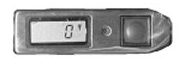
\includegraphics[width=0.7\textwidth]{AAD-Cypres.jpg}\captionof{figure}{Cypres-automaattilaukaisimen käyttöyksikkö}\end{Figure} 

\section{ Muut hyppytoiminnassa käytettävät varusteet }
\label{laskuvarjokalusto-ja-hyppyvarusteet-muut-hyppytoiminnassa-kaytettavat-varusteet}

\begin{itemize}
\item  Kova kypärä, jossa kiinnityshihna on kypärän ulkopuolella. 
\item  Radiovastaanotin on oltava ainakin kolmella ensimmäisellä hypyllä. 
\item  Suojalasit suojaavat silmiä viimalta ja roskilta. 
\item  Haalari, jossa ei saa olla tarttuvia taskuja tai ulokkeita, jotka voivat takertua johonkin tai joista hyppääjä voi vahingossa ottaa kiinni kahvoista kiinni ottaessaan. Haalarin alle puetaan säähän sopiva vaatetus, joka ei haittaa liikkumista. 
\item  Sormikkaat ovat pakolliset oppilailla. Niiden on oltava lämpimät, mutta ei liian paksut eikä liukkaat. 
\item  Kengät, joiden on oltava hyppytoimintaan soveltuvat (ei koukkuja tms.). 
\item  Korkeusmittari, joka nollataan maassa. Mittari kiinnitetään rintahihnaan tai käteen. 
\item  Koukkupuukkoa käytetään takertumien selvittämiseen sotkeutumis- tai törmäämistilanteissa. 
\item  Pelastusliivi puetaan koulutuspäällikön harkinnan mukaan, jos hyppypaikalla on ilmeinen hukkumisvaara. 
\end{itemize}

Hypyn aikana mukana ei saa olla mitään tarpeetonta (esimerkiksi avaimet, kynä tai matkapuhelin). Lisäksi aina hyppäämään tultaessa on oltava mukana hyppypäiväkirja. 

\section{ Hyppyvarusteiden käsittely }
\label{laskuvarjokalusto-ja-hyppyvarusteet-hyppyvarusteiden-kasittely}


Suojaa varjoa auringonvalolta, kosteudelta ja likaantumiselta. Nosta valjaita olkahihnoista ja varo tarttumasta aukaisukahvoihin sekä vaijereiden suojaputkiin. Varjoa ei tule heitellä, laahata eikä sen päällä tule istua. Älä tupakoi, kun olet pukenut valjaat päälle. 


Oppilaan päävarjon pakkaamista saa valvoa henkilö, jolla on itsenäisen hyppääjän kelpoisuus. Oppilaan käytössä olevan päävarjon pakkauksista ja pakkaustarkistuksista pidetään kirjaa. Varavarjon saa pakata vain siihen koulutuksen saanut henkilö. Varusteet palautetaan aina hypyn jälkeen omille paikoilleen. 

\section{ 3X3 -tarkastus }
\label{laskuvarjokalusto-ja-hyppyvarusteet-3x3-tarkastus}


Peruskoulutusvaiheessa oppilaalle opetetaan varusteiden perusteellinen tarkastus, mutta itseaukaisuvaiheessa varjon perustarkastus voidaan tiivistää 3X3 -tarkastukseen (kolme kolmea -tarkastus): 

\begin{enumerate}[label=\bfseries \arabic*)]
\item  Tarkastetaan, että solkia on kiinni kolme: 
	\begin{itemize}
	\item  Vasemman jalkahihnan solki 
	\item  Oikean jalkahihnan solki 
	\item  Rintahihnan solki 
	\end{itemize}
\item  Tarkastetaan, että kahvoja on kolme ja ne ovat kiinni: 
	\begin{itemize}
	\item  Päävarjon avauskahva 
	\item  Päävarjon irtipäästöpampula 
	\item  Varavarjon avauskahva 
	\end{itemize}
\item  Tarkastetaan, että kolmirengaslukot ovat kiinni ja oikein. 
\end{enumerate}
